% this document is part of the DoCrimes project.
% Copyright 2022 the authors

% ## style notes
% --------------
% - quasar sample and random catalog? Or quasar catalog and random catalog? Or different?

% ## to-do items
% --------------
% - test the cmb dipole; cite Secrest et al. NO -- ABBY's PAPER -- BUT DISCUSS THIS POINT.
% - explain, justify, or change how DD, DR, RD, and RR are counted -- the asymmetry between the tree and the sample compared to the tree.
% - discuss more philosophically why alms are sensitive tests of anisotropy
% - make some figure that quantitatively checks Gaia calibration
% - put the expectation hatN_DD onto the non-divided cumulative number plot
% - put in all missing references
% - address all CITE, XXX, YYY, ZZZ, HOGG, KSF in the text
% - make sure the figure axis labels and figure captions use precisely the math symbols used in the text; maybe also turn on TeX in matplotlib?

\documentclass[modern]{aastex631}
\usepackage[utf8]{inputenc}
\usepackage{amsmath}

% typesetting issues
\setlength{\parindent}{3.5ex}
\sloppy\sloppypar\raggedbottom\frenchspacing
\renewcommand{\twocolumngrid}{} % oh yes I can do that

% figure issues
\usepackage[framemethod=tikz]{mdframed}
\usetikzlibrary{shadows}
\definecolor{captiongray}{HTML}{555555}
\mdfsetup{%
  innertopmargin=2ex,
  innerbottommargin=1.8ex,
  linecolor=captiongray,
  linewidth=0.5pt,
  roundcorner=5pt,
  shadow=true,
  shadowcolor=black!05,
  shadowsize=4pt
}
\newlength{\widefigurewidth}
\setlength{\widefigurewidth}{0.95\textwidth}
\newlength{\figurewidth}
\setlength{\figurewidth}{0.75\textwidth}

% math definitions
\newcommand{\unit}[1]{\mathrm{#1}}
\newcommand{\Gpc}{\unit{Gpc}}
\newcommand{\mg}{\unit{mag}}

% text definitions
\shortauthors{hogg and storey-fisher}
\shorttitle{testing isotropy and homogeneity}
\newcommand{\documentname}{\textsl{Article}}
\newcommand{\sectionname}{Section}
\newcommand{\secref}[1]{\sectionname~\ref{#1}}
\newcommand{\figref}[1]{\figurename~\ref{#1}}
\newcommand{\abby}[1]{\textbf{Abby says: #1}}
\newcommand{\hogg}[1]{\textbf{Hogg says: #1}}

\begin{document}

\title{\large%
Testing cosmic isotropy and homogeneity \\ with the \textsl{Quaia} all-sky spectroscopic sample of quasars}
\author[0000-0003-2866-9403]{David W. Hogg}
\affil{Center for Cosmology and Particle Physics, Department of Physics, New York University}
\affil{Max-Planck-Institut f\"ur Astronomie}
\affil{Flatiron Institute, a division of the Simons Foundation}

\author[0000-0001-8764-7103]{Kate Storey-Fisher}
\affil{Center for Cosmology and Particle Physics, Department of Physics, New York University}

\date{2023 July}

\begin{abstract}\noindent
All cosmological models in general relativity are built on the assumption of large-scale isotropy and homogeneity.
These assumptions are testable.
Tests of cosmic isotropy and homogeneity are also strong tests of the quality of data or catalogs and their calibration.
Test precision increases as observations cover more solid angle, become more sensitive to distant objects, and are made with more uniform data.
The ESA \textsl{Gaia} Mission is primarily concerned with stars in the Milky Way, but it also observes millions of quasars, all sky (modulo Galactic extinction), to redshifts of around $4$.
It has produced the largest-comoving-volume public quasar catalog to date.
Here we use the $755\,850$ quasars in the \textsl{Quaia} $G<20.0$ all-sky quasar sample, built from \textsl{Gaia} and \textsl{unWISE} catalogs, to show that the angular distribution, redshift distribution as a function of hemisphere, amplitude of clustering as a function of sky position, and counts of pairs as a function of separation (fractal dimension), are all consistent with large-scale isotropy and homogeneity at the precision possible given the size of the catalog and the amplitude of the large-scale structure.
Roughly speaking, the results can be summarized by saying that they show the Universe to be isotropic at the sub-percent level and homogeneous in the sense of having a fractal dimension of $3.002\pm 0.002$.
There is no sign of any North--South density or power asymmetry.
\abby{Is this the same hemispherical power asymmetry claimed from the CMB?}
\hogg{No, unfortunately; I will do that split too.}
The isotropy results can also be interpreted as a strong test of the spectrophotometric uniformity of the \textsl{Quaia} Catalog.
\end{abstract}

\keywords{%
calibration
---
catalogs
---
cosmic~isotropy
---
cosmological~principle
---
cosmology
---
large-scale~structure~of~the~Universe
---
quasars
}
\section*{}
\clearpage
\section{Introduction}\label{sec:intro}\noindent
One of the fundamental assumptions of the physical cosmological model is that the Universe is isotropic and homogeneous on large scales (for example, \citealt{peebles, ryden}).
This assumption is testable.
It is worthy of test, both because it is always worth testing fundamental assumptions, and because the large-scale structure has self-similar or fractal characteristics, which are characteristic of inhomogeneous distributions.
And, even in the ascendent physical model of cosmology, there is expected to be at least some power in the initial conditions on all length scale.

If the Universe failed tests of homogeneity on large scales, and in particular if the Universe turned out to be a fractal with a fractal dimension significantly less than 3, we would be in big trouble theoretically.
Why?
Because a fractal universe has no well-defined mean density.
There are no working physical models for such an inhomogeneous universe.
Indeed, there are not even any known solutions of the equations of general relativity without a well-defined mean density.

All that said, we know now that the Universe is not a fractal on large scales (\citealt{hogg05}; CITE OTHERS).
There are other reasons to continue to test isotropy and homogeneity however.
One is that the cosmic microwave background appears to show a power asymmetry, in which there appears to be a larger amplitude of fluctuations in the North/South Ecliptic (\hogg{this is not quite right, or is it?}) Cap than there is in the South/North (\citealt{wmapanisotropy}; \citealt{planckanisotropy}).
If this asymmetry is real, it should show itself in the large-scale structure as well (\citealt{zhai}).

Another reason to make new tests of isotropy and homogeneity is that data samples keep getting larger in volume and number, permitting more and more sensitive tests.
Here we make use of the brand-new \textsl{Quaia} catalog of quasars.
This catalog is built from the ESA \textsl{Gaia} DR3 data (CITE), which includes more than a million quasars, all-sky (CITE), plus photometry from the \textsl{unWISE} catalog (CITE), which is built on the NASA \textsl{WISE} infrared imaging.
This data set is not the largest cosmological data set in terms of number of tracers, but it is the largest-ever data set in terms of comoving volume, spanning some XXX $h^{-3}\,\Gpc^3$ (comoving), depending on how you want to define the sample volume.
Recent tests of homogeneity include ZZZ and ZZZ; the samples used in those studies were smaller by a factor of QQQ and WWW (approximately) in comoving volume, relative to the quasar catalog we use here.

A final but equally important reason to test isotropy and homogeneity is that these tests provide a very strong validation of the quality and uniformity of the data.
Indeed, the first work on homogeneity with the Sloan Digital Sky Survey data (\citealt{hogg05}) was performed to test the calibration and stability of the data in preparation for the measurement of the baryon acoustic feature (\citealt{baf}).
The work presented here represents a first strong test of the calibration of the \textsl{Quaia} quasar sample and associated photometry and spectroscopy; it has implications for the accuracy and uniformity of the \textsl{Gaia} data more generally.

\section{Data}\label{sec:data}\noindent
\hogg{Make sure we cite the CU5 papers and XP papers here and anything that helped make the extragalactic and quasar samples.}

The data used in this project is the XXX quasar sample (\citealt{ksf}), derived from the ESA \textsl{Gaia} quasar candidate catalog (CITE).
This candidate catalog was released as part of the \textsl{Gaia} Data Release 3 data (DR3; CITE).
The catalog was constructed using the overlap of the \textsl{Gaia} DR3 data with photometry from the NASA \textsl{WISE} Mission (CITE), and spectro-photometric redshifts were estimated using a combination of XXX photometry, \textsl{Gaia} DR3 \texttt{qsoc} (maybe?) redshift estimates, and a training set from \textsl{SDSS-IV} Data Release 17 data (CITE).
For more information see the XXX quasar catalog paper (\citealt{ksf}).

\begin{figure}[t!]
  \begin{mdframed}
  \color{captiongray}
  \begin{center}
    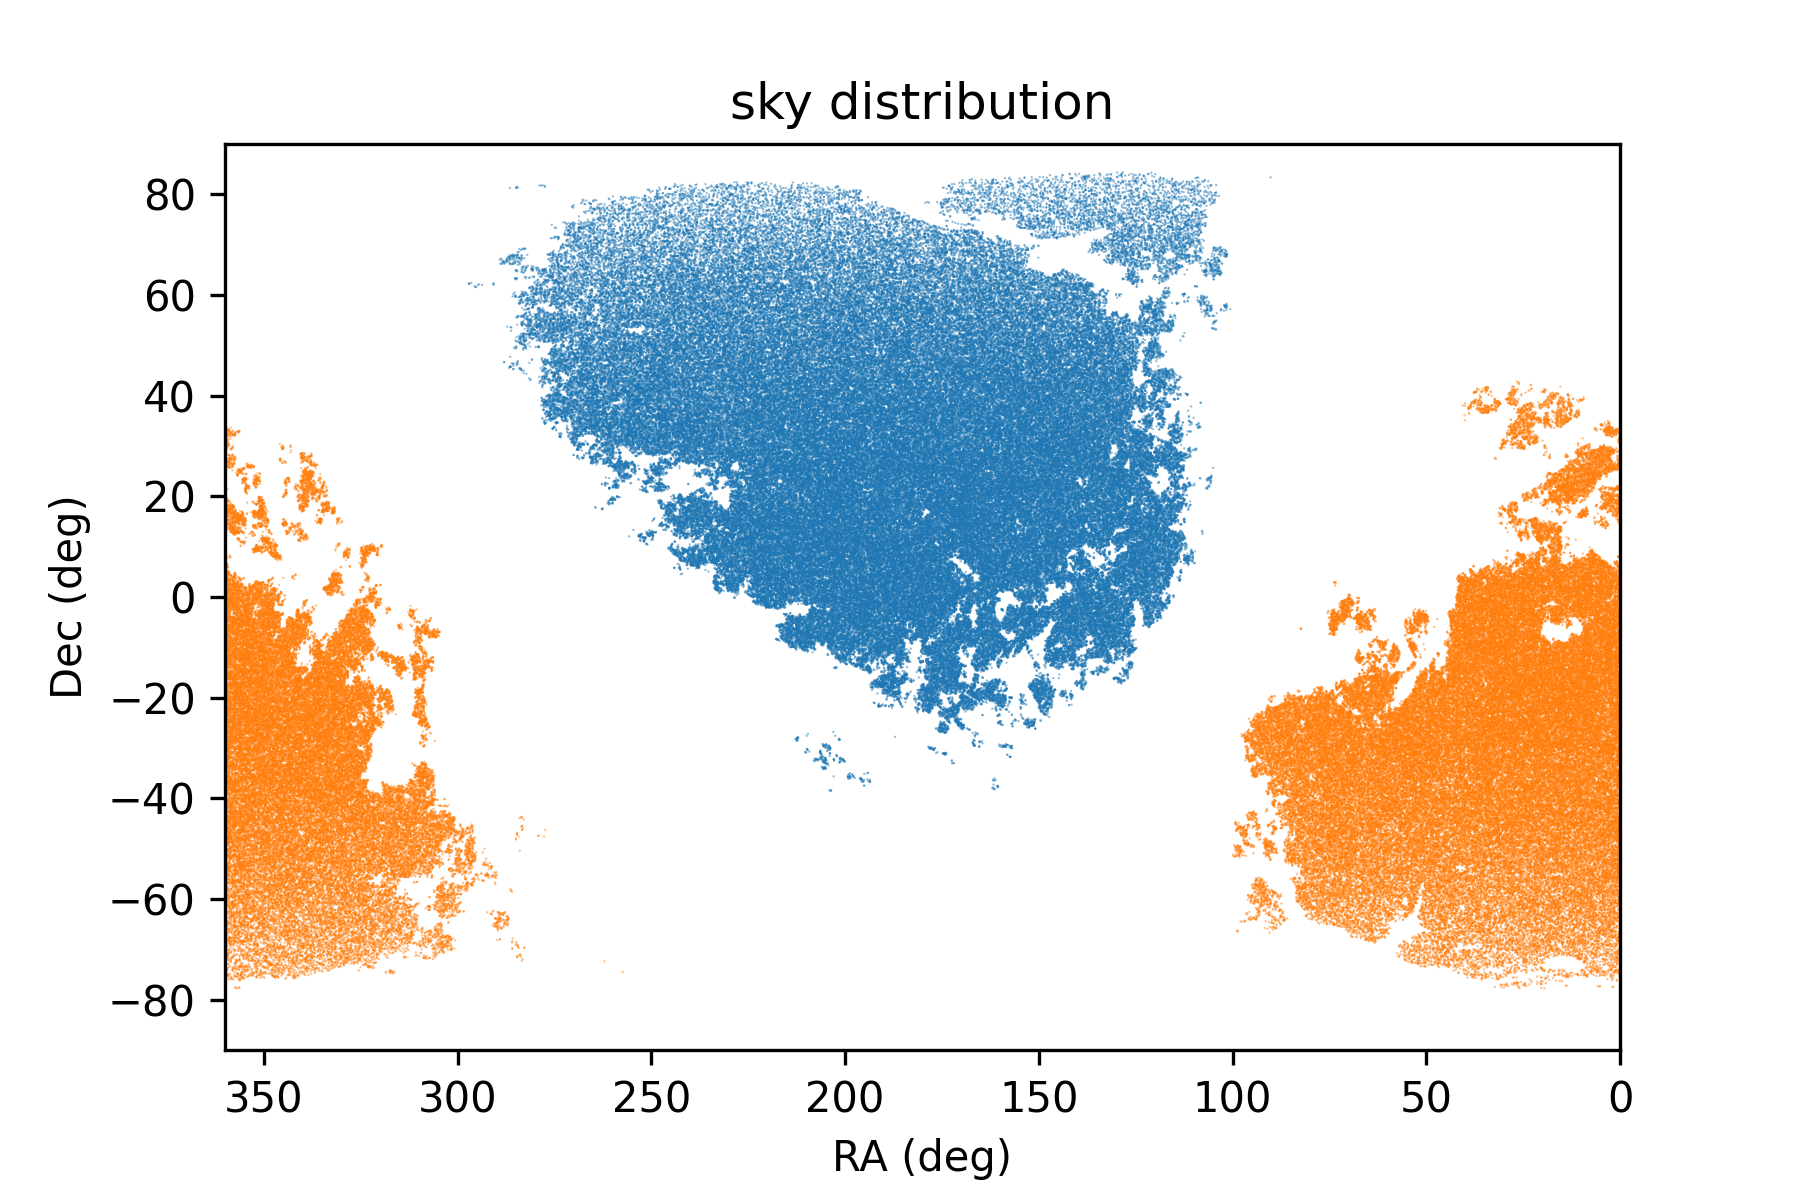
\includegraphics[width=\figurewidth]{notebooks/radec.png}
  \end{center}
    \caption{The full quasar sample, obtained after cutting on apparent magnitude and extinction, plotted on the sky in Equatorial coordinates.
    The NGC subsample (and its associated random catalog) is colored blue and the SGC subsample is colored orange.
    Stars from the Bright Star Catalog (\citealt{bsc}) with $V<4\,\mg$ are shown as grey disks for angular reference.\label{fig:radec}}
  \end{mdframed}
\end{figure}
We cut the full XXX quasar sample to \textsl{Gaia} $G<20\,\mg$ for redshift reliability.
We further cut it to an infrared-emission-based extinction estimate of YYYY$<$whatever (\citealt{sfd}) for angular uniformity.
Finally, we tag those quasars with Galactic latitude $b>0$ ``North Galactic Cap'' (NGC) and those with $b<0$ ``South Galactic Cap'' (SGC).
These cuts leave XXX quasars in the sample, YYY in the NGC subsample and ZZZ in the SGC subsample.
The sample is shown on the sky in the equatorial coordinate system in \figref{fig:radec}.

\begin{figure}[t!]
  \begin{mdframed}
  \color{captiongray}
  \begin{center}
    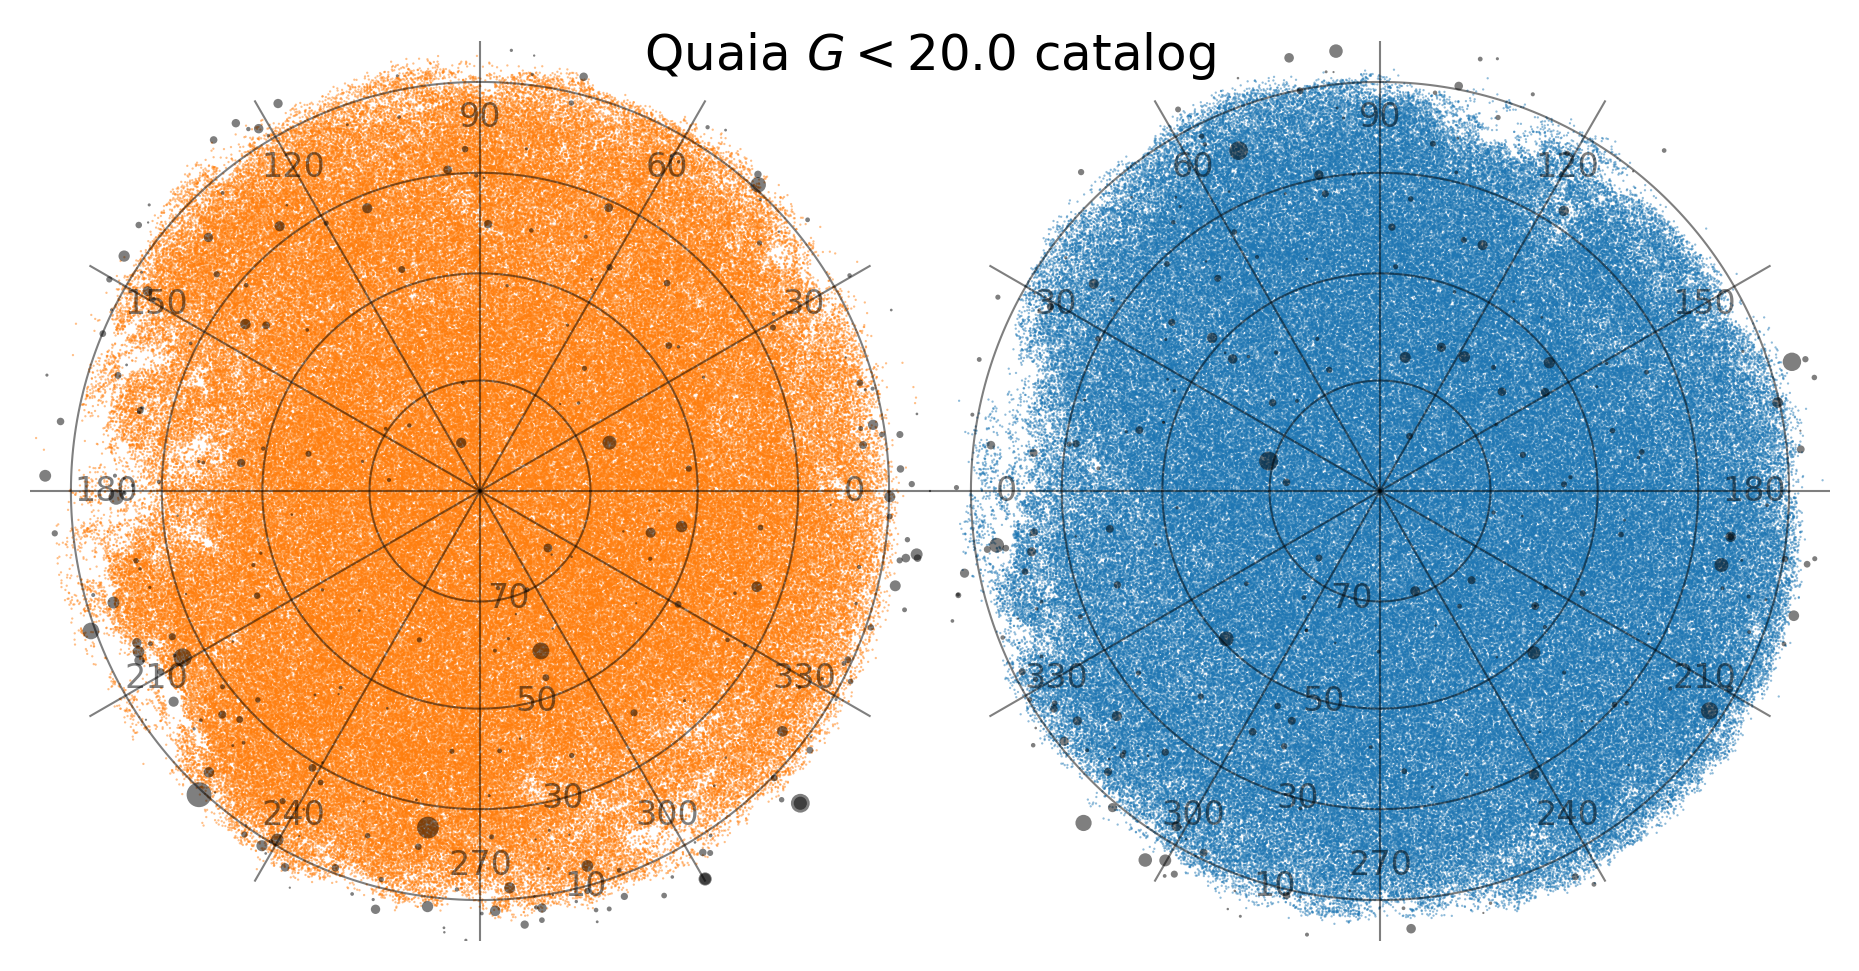
\includegraphics[width=\figurewidth]{notebooks/lb.png}\\
    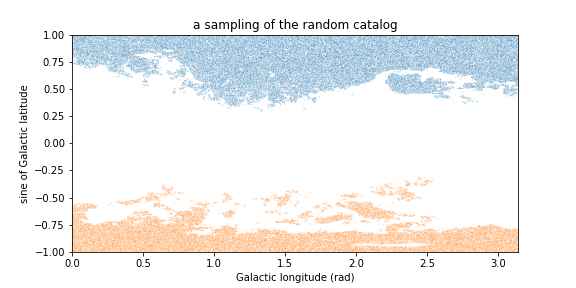
\includegraphics[width=\figurewidth]{notebooks/lb_random.png}
  \end{center}
    \caption{The full quasar sample obtained after cutting on apparent magnitude and extinction (top) and a sampling of the much larger random catalog obtained after making those same cuts (bottom), plotted on the sky in Galactic coordinates.
    This projection is designed to be equal-area (the Lambert azimuthal equal-area projection), such that a set of quasars uniformly distributed on the sky would make a set of points uniformly distributed on this 2-d plot.
    The NGC subsample (and its associated random catalog) is colored blue and the SGC subsample (and its associated random catalog) is colored orange.
    Stars from the Bright Star Catalog (\citealt{bsc}) with $V<4\,\mg$ are shown as grey disks for angular reference.\label{fig:lb}}
  \end{mdframed}
\end{figure}
The XXX quasar catalog comes with an associated random catalog with a near-identical sky footprint but YYYY times the density (\citealt{ksf}).
The random-catalog footprint is modulated by stellar density and Galactic extinction, with these modulations fit to match the observed data.
We cut the random catalog identically to the quasar catalog.
Both the quasar catalog and an equivalent-density sampling of the random catalog are shown on the sky in the Galactic coordinate system in \figref{fig:lb}.

\hogg{Make sure to explain somewhere how the random catalog points get redshifts!!}

\section{Isotropy}\label{sec:iso}\noindent
A simple kind of isotropy is evident in \figref{fig:lb}:
Because the sky plots shown there are equal-area projections, the uniformity of the sample in those plots is an indicator of isotropy.
This observation can be made more quantitative by projecting onto spherical harmonics.
In detail, we project onto the spherical harmonics by
\begin{equation}\label{eq:alms}
    a_{\ell m} = \sum_n Y_{\ell m}(\Omega_n) ~,
\end{equation}
where $a_{\ell m}$ is a spherical-harmonic amplitude,
$\ell, m$ are the angular degree and order,
$n$ is an integer index and the sum is over all quasars,
$Y_{\ell m}(\Omega)$ is the spherical harmonic at degree $\ell$ and order $m$,
and
$\Omega_n$ is the sky position (Galactic $l, b$) for quasar $n$.
The spherical harmonics are oriented in the natural way in the Galactic coordinate system, such that $Y_{10}$ has a maximum in the direction of the Galactic Center.
The top panel of \figref{fig:alms} shows these amplitudes $a_{\ell m}$.
The amplitudes $a_{\ell m}$ are complex, so \figref{fig:alms} shows the real and imaginary parts of the $m\geq 0$ orders.

\begin{figure}[t!]
  \begin{mdframed}
  \color{captiongray}
  \begin{center}
    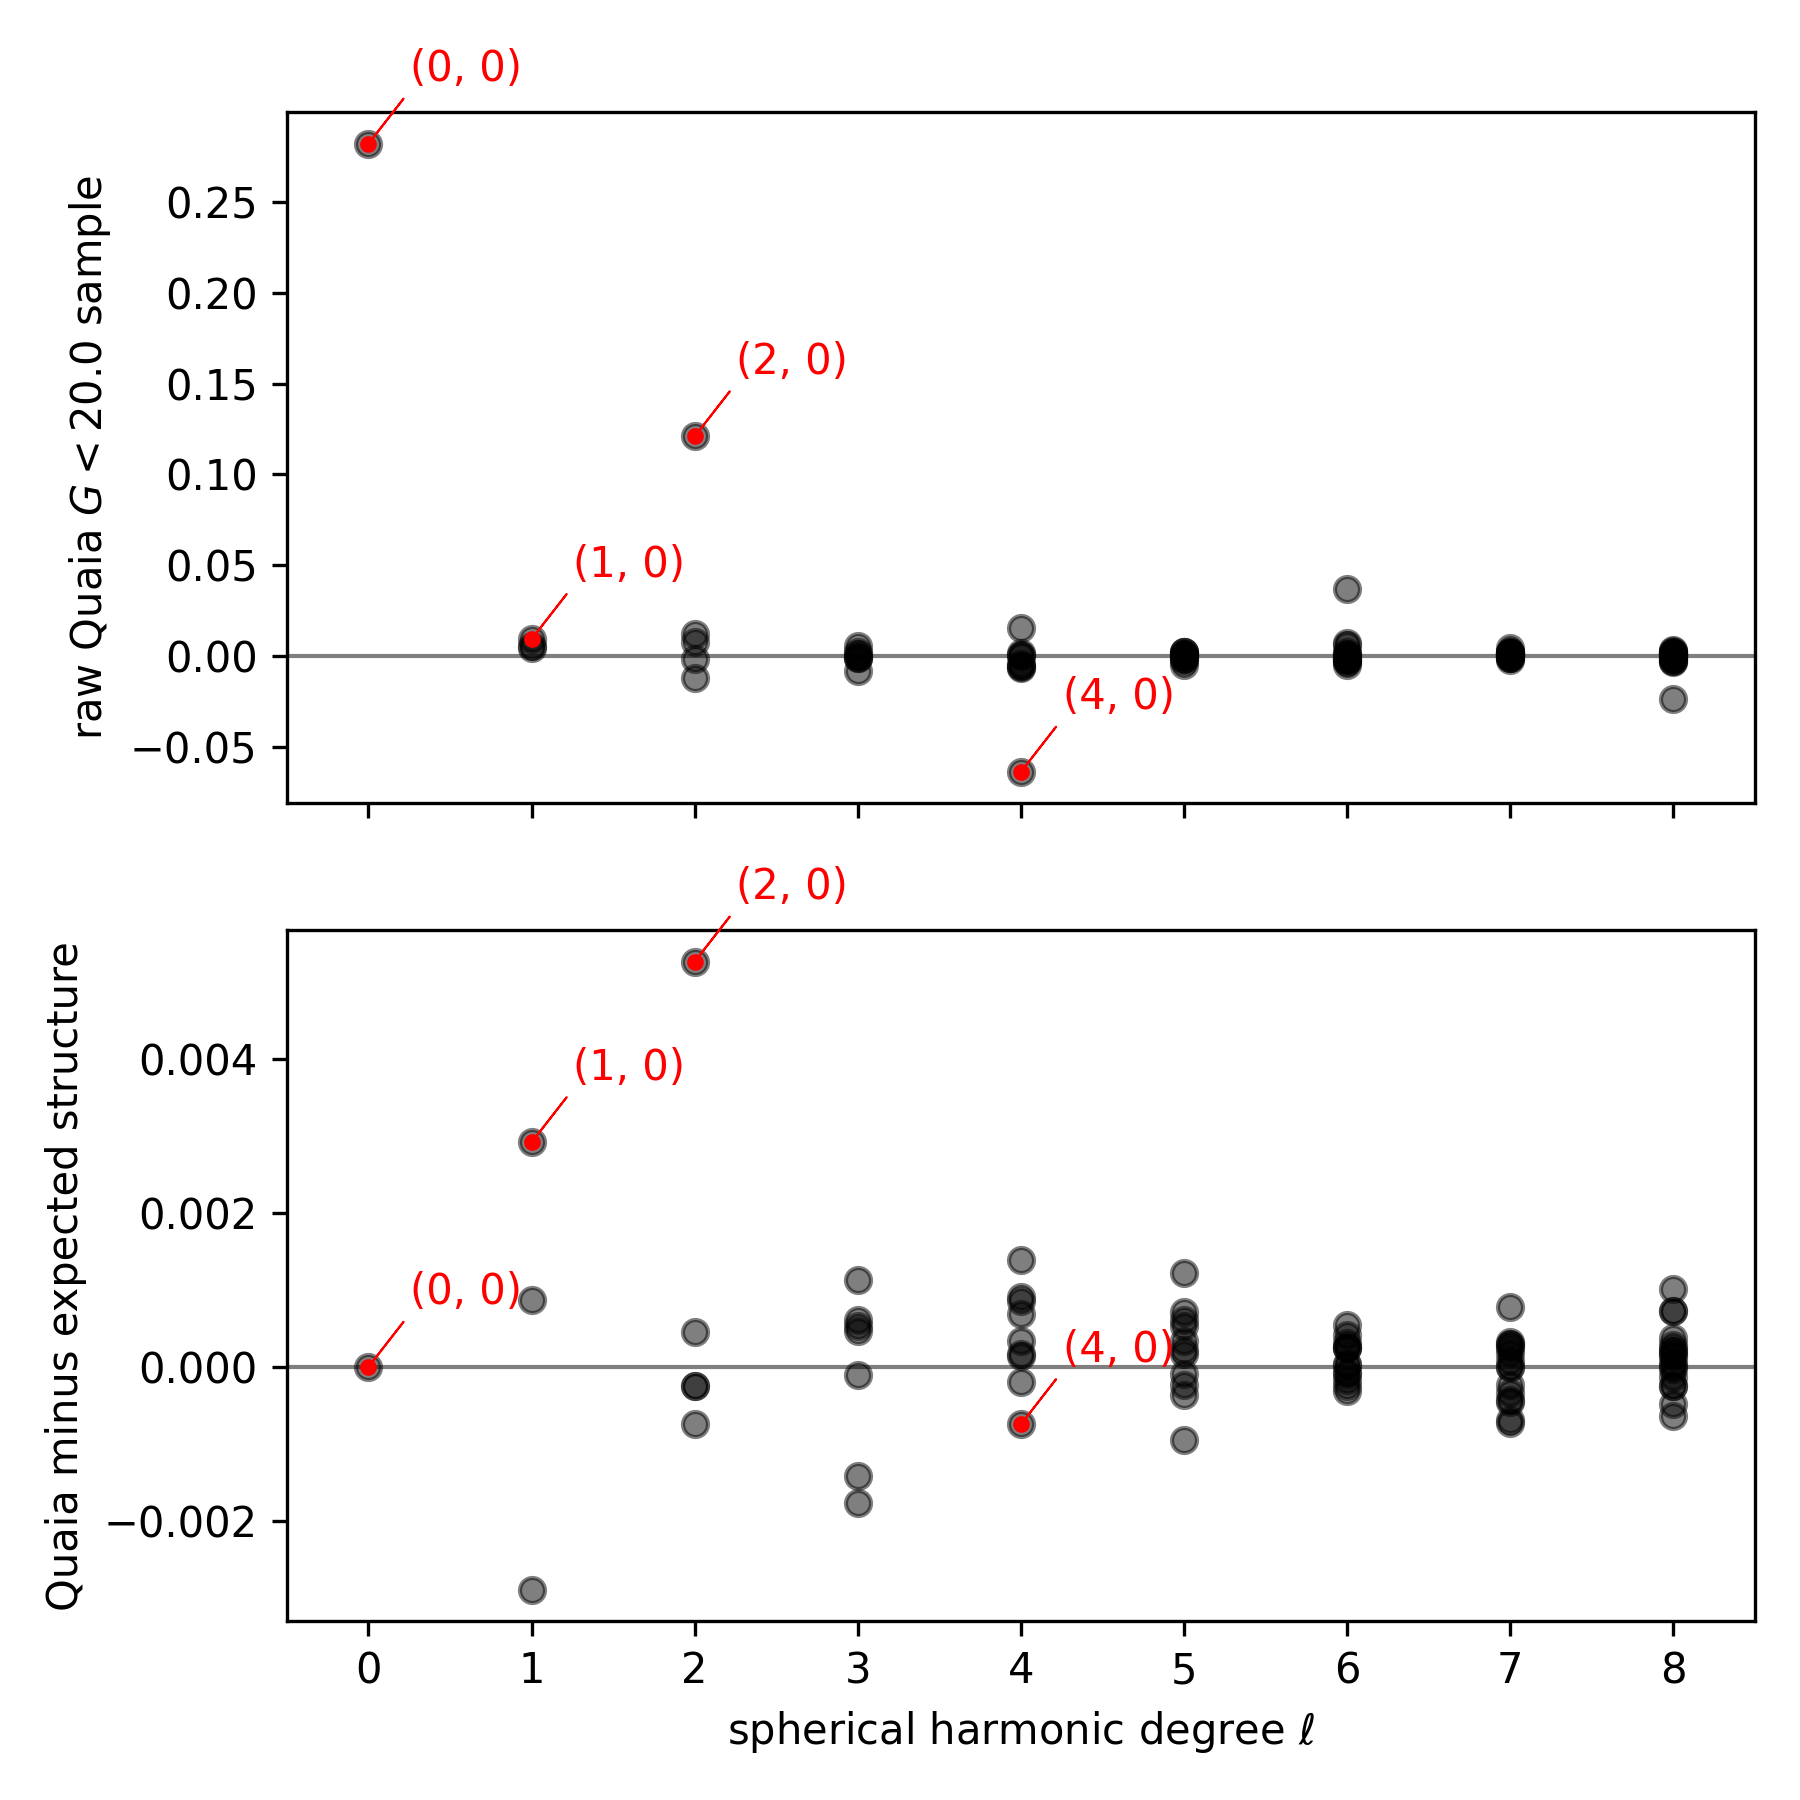
\includegraphics[width=\figurewidth]{notebooks/alms.png}
  \end{center}
    \caption{The spherical-harmonic expansion for the sky distribution, in the natural Galactic coordinate-system spherical harmonics. \textsl{Top:} The real and imaginary amplitudes of the spherical-harmonic expansion for the data set. It has a large amplitude at $(\ell,m)=(2,0)$ because of the quadrupolar form of the extinction map (and therefore sample selection). \textsl{Bottom:} The same, but the real and imaginary amplitudes for $\ell>0$ have been adjusted for their expectation under the selection function, as it has been represented by the random catalog. The low amplitudes at $\ell>0$ in the bottom panel demonstrate the isotropy of the sample. There are still residual amplitudes at $(\ell, m)=(1,0)$, $(2,0)$, and $(4,0)$ as expected if there are small issues with the completeness model (selection function model), which is based on an extinction map and a stellar-density map.\label{fig:alms}}
  \end{mdframed}
\end{figure}
There is clear anisotropy visible in the top panel of \figref{fig:alms}, in the form of non-zero amplitudes at $\ell>0$.
However, the anisotropic structure can be explained by the selection function.
The bottom panel of \figref{fig:alms} shows the amplitudes again, but after the $\ell>0$ amplitudes have had their expectations subtracted.
Their expectations are computed by performing the same sums as in \eqref{eq:alms}, but with the random catalog instead of the quasar catalog.
These represent the expectations under isotropy because the random catalog is made with a perfectly isotropic distribution cut by an estimate of the selection function.

In detail, the selection function was inferred (and the random catalog was made) using an empirical procedure that essentially assumes that the quasar sample is isotropic (see \citealt{ksf} for details).
Does this make the test shown in \figref{fig:alms} circular or true by assumption?
It does not, because the only freedoms permitted in constructing the random catalog were dependences on observed extinction (according to the infrared-emission map of \citealt{sfd}) and the stellar density (according to a count of stars in the \textsl{Gaia} catalog).
And, indeed, the biggest anisotropic amplitudes are at $(\ell,m)=(1,0)$, $(2,0)$, and $(4,0)$, which are exactly what are expected if this completeness map is not perfect:
The dust extinction map and the stellar extinction map have most of their power in these modes (because we live in a disk Galaxy but do not live at its Center).

\begin{figure}[t!]
  \begin{mdframed}
  \color{captiongray}
  \begin{center}
    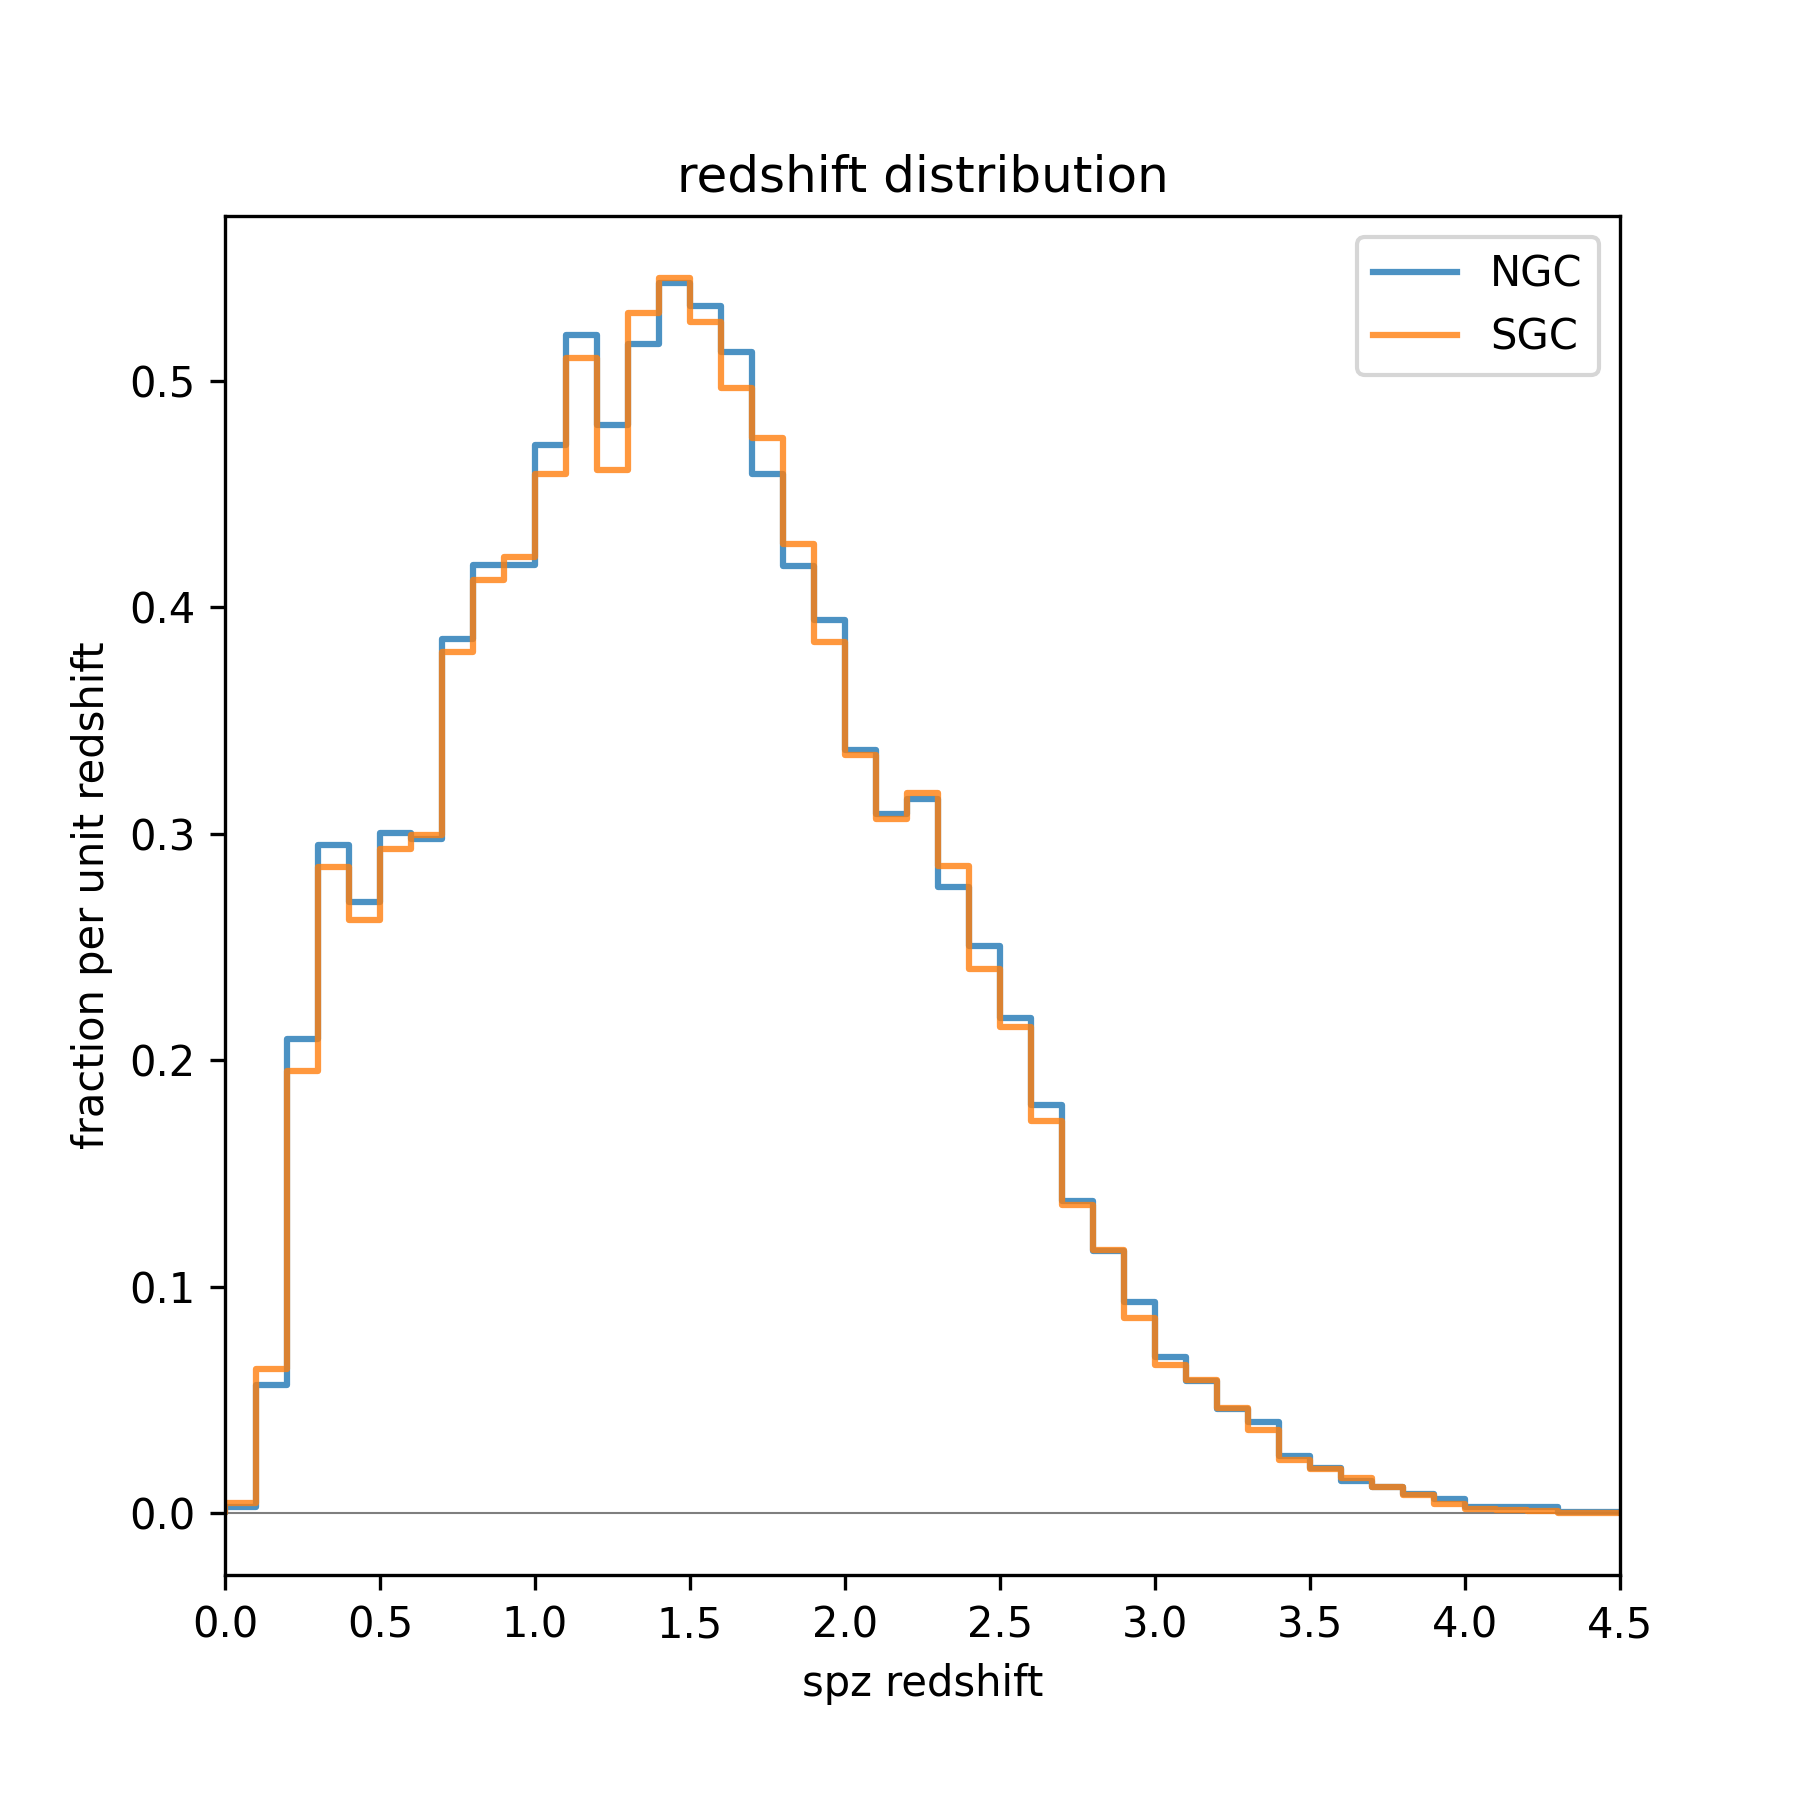
\includegraphics[width=\figurewidth]{notebooks/zhist.png}
  \end{center}
    \caption{The redshift distributions of the NGC and SGC subsamples. This demonstrates that the distribution of quasar spectrophotometric properties is very similar between the North and South.\label{fig:zhist}}
  \end{mdframed}
\end{figure}
HOGG: Another strong test of isotropy can be obtained from the redshift distribution.
Why is this strong?
It also connects to the hemispherical power asymmetry in the CMB (\citealt{wmapanisotropy}; \citealt{planckanisotropy}).

HOGG: In principle we could do something that is even more extreme, which would be the projection of the redshift distribution onto spherical harmonics. Anyone up for that? Might discover non-seperability of the angular and redshift distributions.

\section{Homogeneity}\label{sec:homo}\noindent
The weakest possible prediction of homogeneity is that there should be a mean density to the Universe.
This prediction is weak, but it has the advantage that it carries few other assumptions.
The prediction that there exists a mean density can be cast in terms of the scaling of pair counts or a measurement of the \emph{fractal dimension}.
The fractal dimension, for a set of points in a space, is defined to be the scaling of the total number of pairs $N_{DD}$ in the set with the maximum separation $s$ out to which pairs are counted.
If $N_{DD}$ is proportional to $s^d$ then the fractal dimension is $d$; if $d=3$ then the Universe has a mean density.

\begin{figure}[t!]
  \begin{mdframed}
  \color{captiongray}
  \begin{center}
    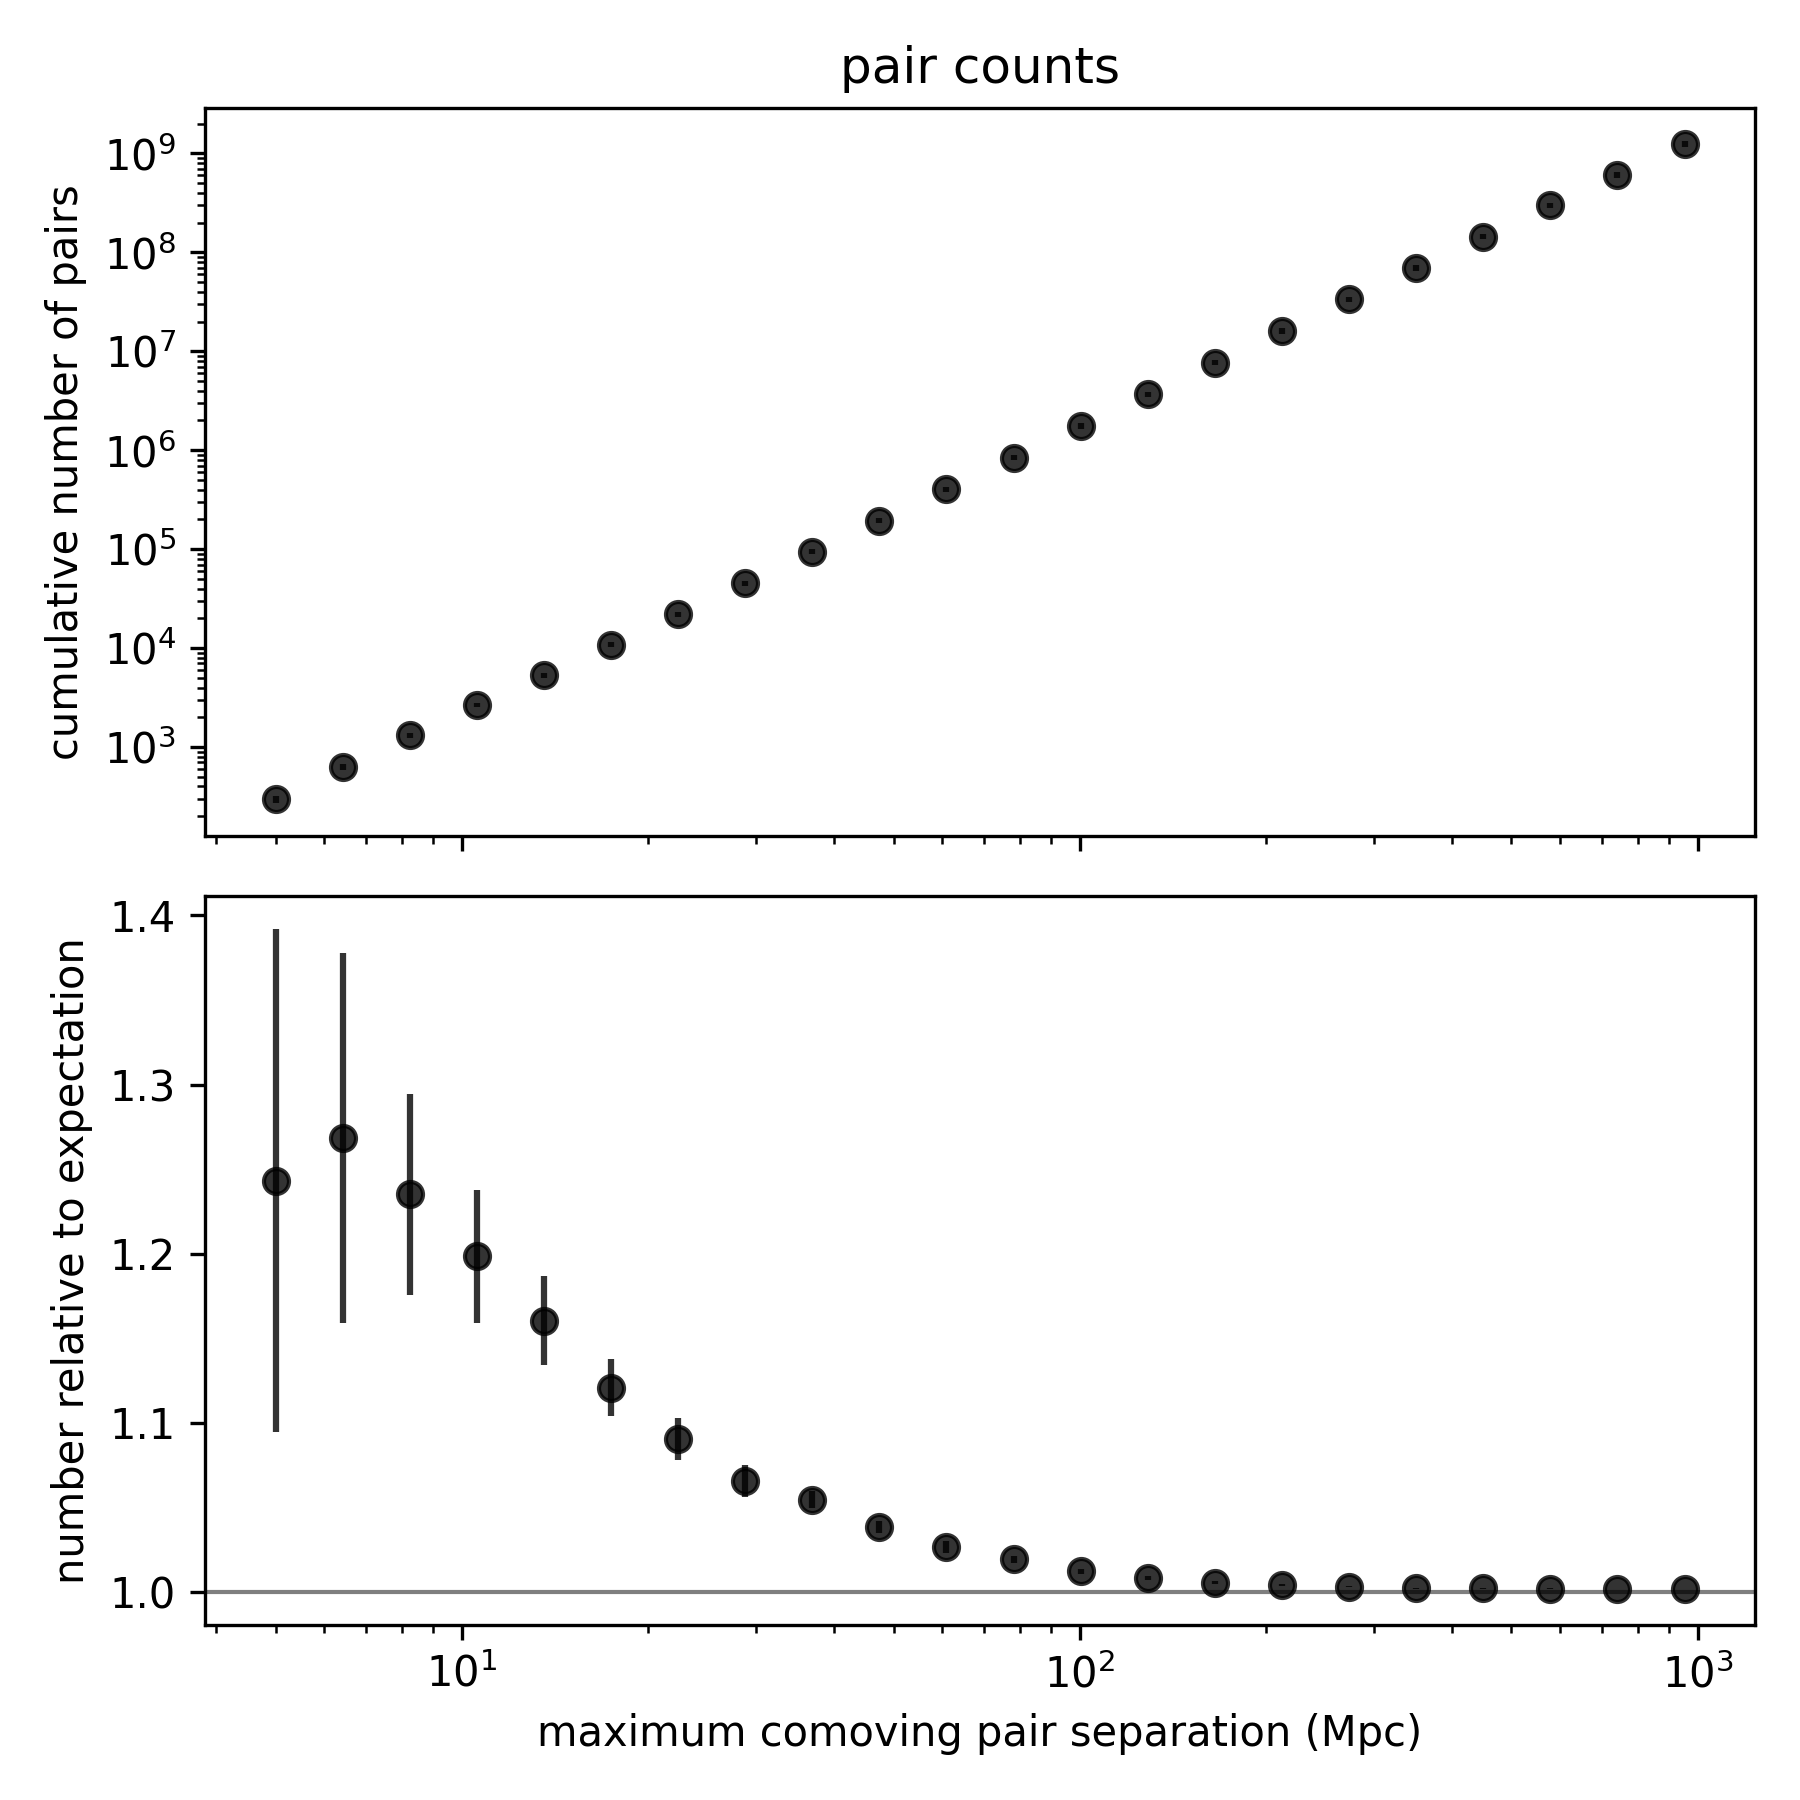
\includegraphics[width=\figurewidth]{notebooks/cumulativeDD_DR.png}
  \end{center}
    \caption{\textsl{Top:} The cumulative total number $N_{DD}$ \eqref{eq:DD} of quasar--quasar pairs as a function of comoving separation $s$ for the NGC and SGC subsamples. Jackknife uncertainty estimates are shown but are smaller than the points for all points.
    \textsl{Bottom:} The same, but divided by the expectation $\hat{N}_{DD}$ \eqref{eq:DDhat} in a homogeneous universe.
    This figure demonstrates that the fractal dimension is extremely close to $3$.
    \hogg{Explain the fractal-dimension label.}\label{fig:cumulative}}
  \end{mdframed}
\end{figure}
The cumulative number $N_{DD}$ of pairs up to separation $s$ is shown as a function of $s$ in the top panel of \figref{fig:cumulative}.
The top panel shows the raw counts of pairs, and the bottom panel shows the pairs relative to an expectation derived from the random catalog, which (by construction) has fractal dimension $d=3$.
Although the scaling in the top panel of \figref{fig:cumulative} looks very good, it can be biased by the finite volume within which we have observations; hence the ratios plotted in the bottom panel of \figref{fig:cumulative}.
In detail, the statistics that are plotted are cumulative pair counts obtained as follows:
We start by counting pairs within the quasar sample, between the quasar sample and the random catalog, and within the random catalog, by
\begin{align}\label{eq:DD}
    N_{DD}(s) &= \sum_n \sum_{n'\ne n} I(r_{nn'} < s) \\
    N_{DR}(s) &= f\,\sum_n \sum_{m'} I(r_{nm'} < s) \\
    N_{RD}(s) &= f\,\sum_m \sum_{n'} I(r_{mn'} < s) \\
    N_{RR}(s) &= f^2\,\sum_m \sum_{m'\ne m} I(r_{mm'} < s)\label{eq:RR} ~,
\end{align}
where the sums over $n$ or $n'$ are over quasars,
the sums over $m$ or $m'$ are over random points,
$r_{nn'}$ is the comoving distance between quasar $n$ and quasar $n'$,
$I(r<s)$ is an indicator function that returns 1 if $r<s$ and 0 otherwise,
and $f$ is a dimensionless ratio of the density of the quasar sample (on the sky) to the density of the random catalog (on the sky).
With these counts in hand, the expectation $\hat{N}_{DD}(s)$ we use for the cumulative pair counts $N_{DD}(s)$ is given by
\begin{equation}\label{eq:DDhat}
    \hat{N}_{DD}(s) = N_{DR}(s) + N_{RD}(s) - N_{RR}(s) ~,
\end{equation}
which is inspired by the currently standard correlation-function estimator (\citealt{ls}).

\hogg{\figref{fig:cumulative} strongly suggests that the fractal dimension $D$ is 3.
Our best-fit value is ... WHAT?
Get quantitative here and explain how we computed the fractal dimension.}

For the maximum separation $s$ and the separations $r_{nn'}$ in \eqref{eq:DD} and the subsequent equations for the pair counts, we used the comoving distance in the \textsl{Planck} 2018 cosmology (\citealt{planck18}).
This is a strong assumption, and wrong if the Universe has no mean density.
Indeed, since (as we note in \secref{sec:intro}) there are no known solutions to the equations of general relativity in an inhomogeneous universe, there is no way to compute pair separation distances $r_{nn'}$ without making the assumption of homogeneity.
The fact that this test passes---that the Universe appears to have a well-defined mean density and looks homogeneous on large scales---is a non-trivial test, but it does have this limitation, which cannot be addressed at present.

In order to put error bars on the counts $N_{DD}$ and its expectation $\hat{N}_{DD}$ (HOGG: DID WE DO THAT?), we performed jackknife resampling.
Because we want the jackknife resampling to estimate uncertainty due not just to shot noise in the sample, but also large-scale structure modes, we performed the jackknife with 12 subsamples, in each of which we left out a disjoint contiguous 1/12 of the sky.
In detail we segmented the sky by galactic longitude $l$, and in each of the 12 leave-1/12-out subsample we re-did the full analysis including all counts of pairs.
The error bars in \figref{fig:cumulative} are estimated by this jackknife.

\section{Statistical isotropy}\label{sec:stat}\noindent
If the fractal dimension is 3, then the correlation function should go to zero at large scales.
It does (CITE THINGS)!
But observations of the cosmic microwave background have suggested that there might be a power asymmetry between the North and South Galactic Caps (CITE).
This asymmetry claim constitutes a claim of statistical anisotropy:
The statistics of the matter distribution depend on direction.
In a homogeneous universe (homogeneous in the sense of having a mean density), that statistical anisotropy, in turn, would imply a statistical inhomogeneity.
Thus it is interesting to check the quasar sample for any evidence for such a statistical anisotropy or statistical inhomogeneity.

The pair counts $N_{DD}(s), N_{DR}(s), N_{RD}(s), N_{RR}(s)$ obtained in \eqref{eq:DD} through \eqref{eq:RR} can be massaged into differential counts (counts within a separation bin) and then used to construct an estimate of the 3-space auto-correlation function of the quasars.
The differential counts $\Delta N_{DD,i}, \Delta N_{DR,i}, \Delta N_{RD, i}, \Delta N_{RR, i}$ in a separation bin $i$ can be defined with differences like
\begin{equation}
    \Delta N_{DD,i} = N_{DD}(s_i+\frac{1}{2}\,\Delta s) - N_{DD}(s_i-\frac{1}{2}\Delta s) ~,
\end{equation}
where $s_i$ is the bin center and $\Delta s$ is the bin width in separation space.
These differential counts can be combined into an estimate $\hat\xi(s_i)$ of the auto-correlation function with the Landy--Szalay estimator (\citealt{ls}):
\begin{equation}\label{eq:ls}
    \hat\xi(s_i) = \frac{\Delta N_{DD,i} - \Delta N_{DR,i} - \Delta N_{RD,i} + \Delta N_{RR,i}}{\Delta N_{RR,i}} ~.
\end{equation}

\begin{figure}[t!]
  \begin{mdframed}
  \color{captiongray}
  \begin{center}
    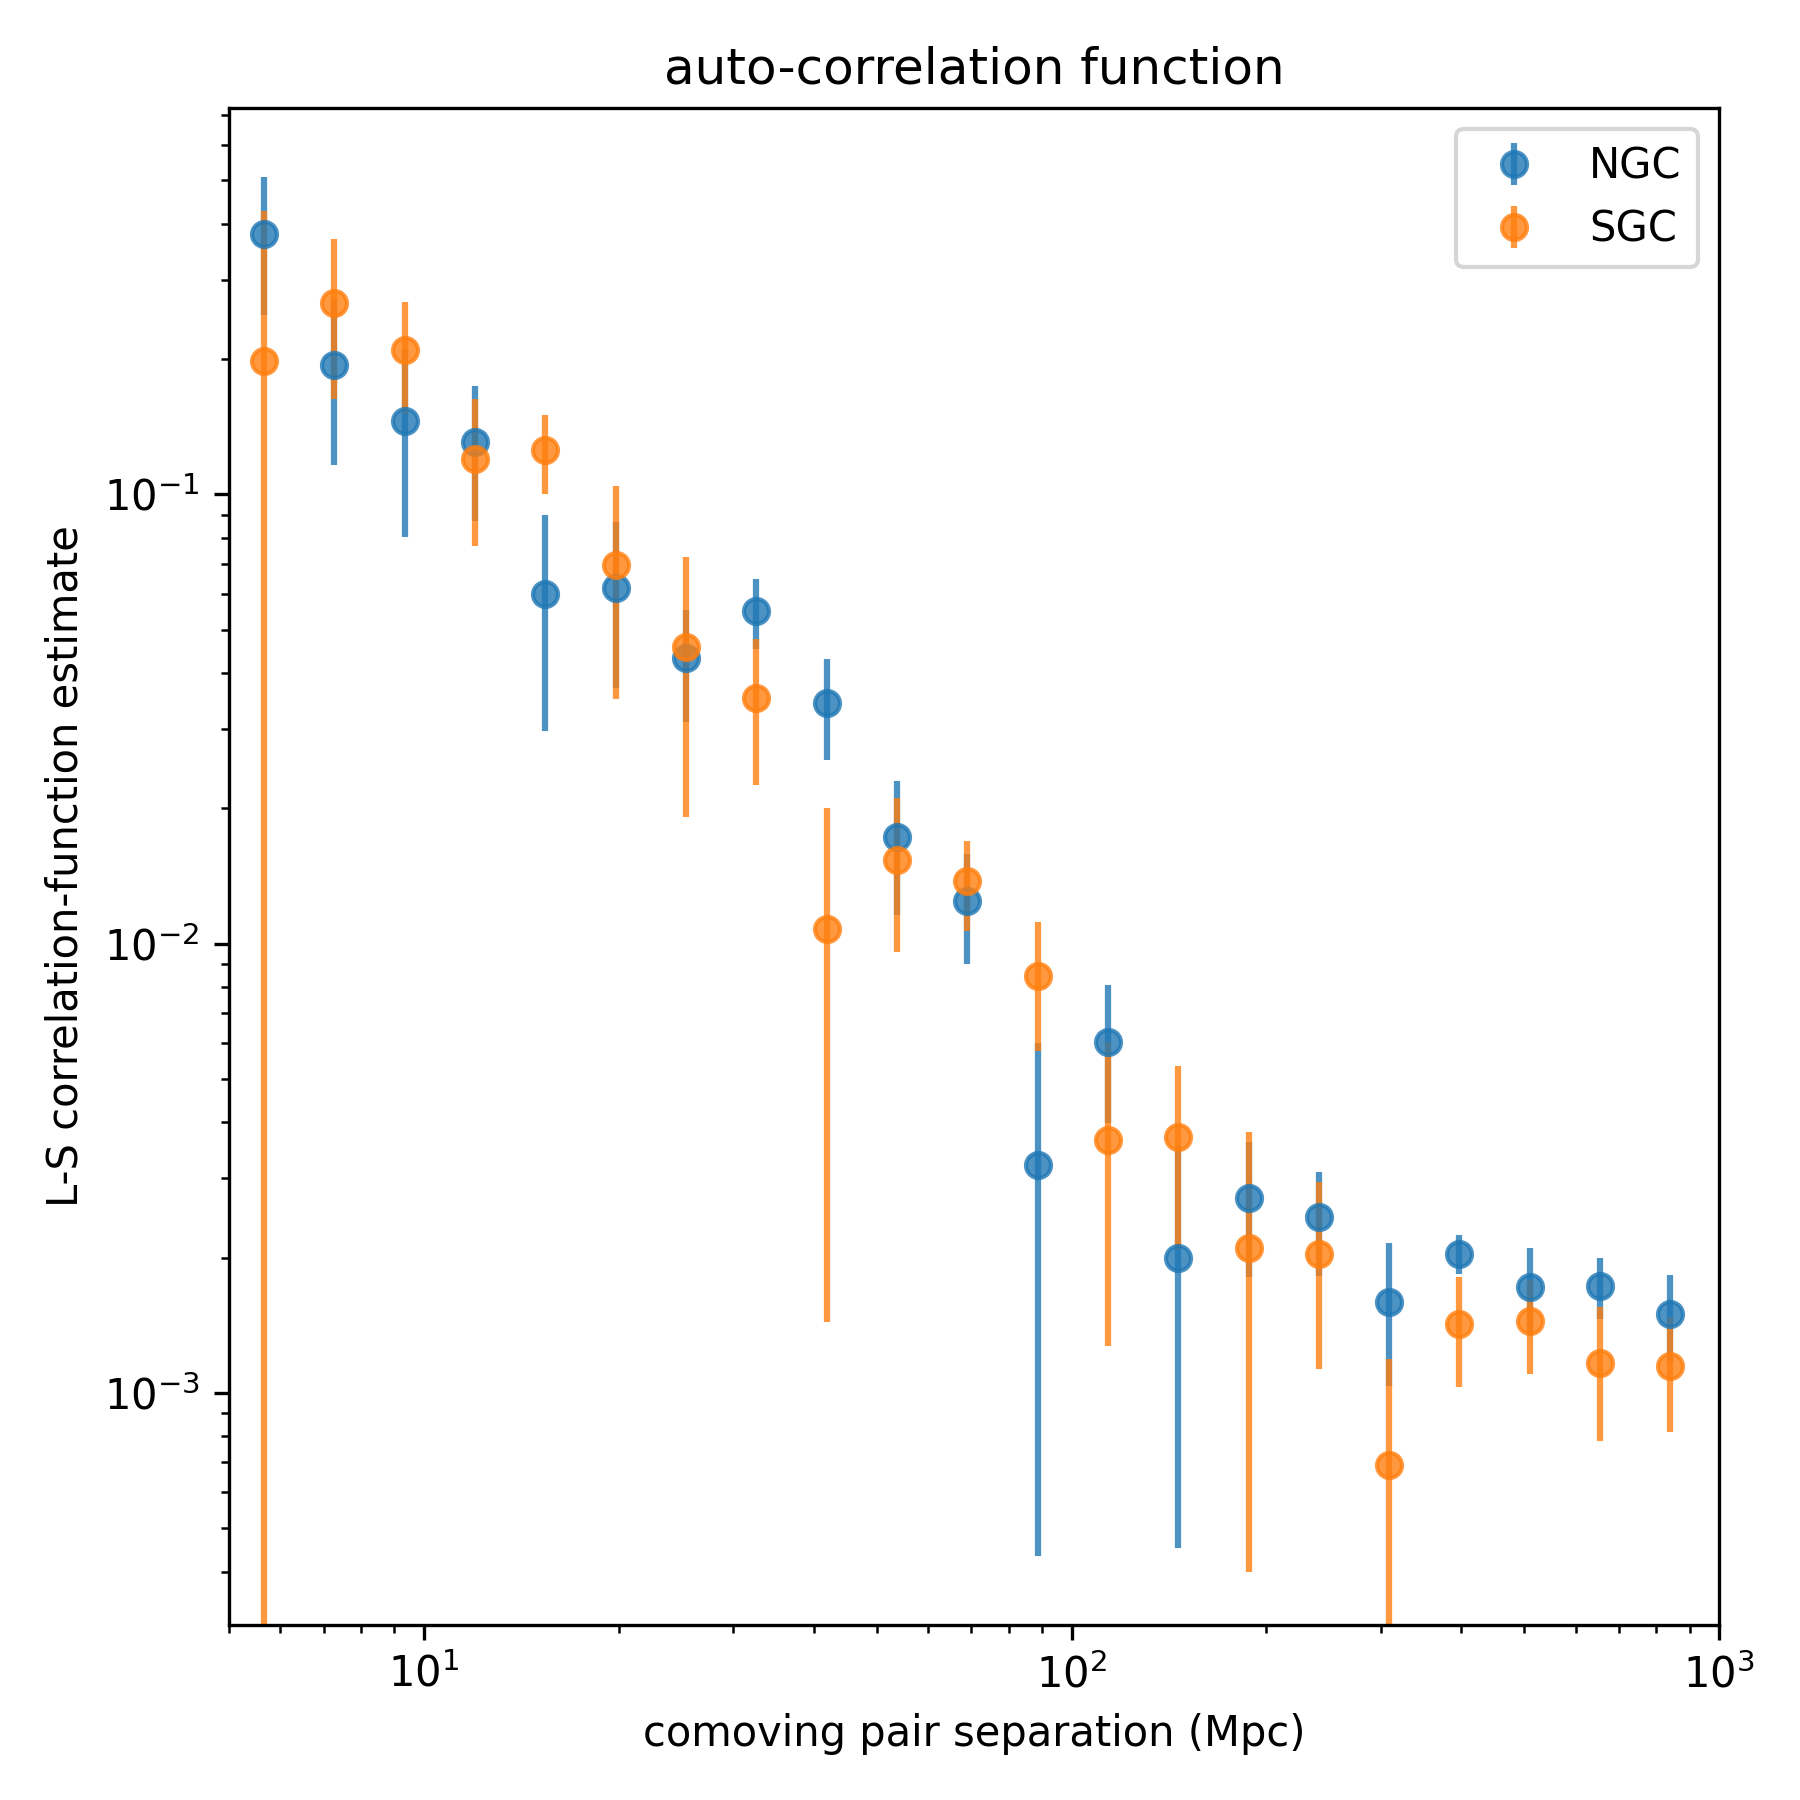
\includegraphics[width=\figurewidth]{notebooks/corrfunc.png}
  \end{center}
    \caption{The auto-correlation of the quasars as a function of comoving separation $s$ for the NGC and SGC subsamples, as estimated according to \eqref{eq:ls}.
    This figure demonstrates that the clustering amplitude is similar between the North and the South.\label{fig:corrfunc}}
  \end{mdframed}
\end{figure}
\figref{fig:corrfunc} shows the quasar auto-correlation function estimated according to \eqref{eq:ls} for the quasar sample in coarse separation bins, separated by sky hemsiphere.
The figure shows that the auto-correlation function is statistically consistent between hemispheres for this sample.
This result does not confirm the hemispherical power asymmetry observed in the cosmic microwave background.
Instead it supports the conclusion that the Universe is statistically isotropic and statistically homogeneous.

\section{Discussion}\label{sec:discuss}\noindent
\hogg{We found what we expected to find, but at very good precision.}

\hogg{How to summarize these results?}

\hogg{Comment on the dipole and surrounding controversy.}

\hogg{What would have been different if we had gone to the $G<20.4$ sample?}

\hogg{Note that the selection function was built by assuming isotropy. In detail, that must bias our results.}

\hogg{What to say about uniformity and calibration of Quaia?}

\begin{acknowledgements}
It is a pleasure to thank
  Anna-Christina Eilers (MIT),
  Hans-Walter Rix (MPIA), and
  Abby Williams (NYU, Caltech)
for valuable discussions.
This project was developed in part at the 2022 Gaia F\^ete, hosted by the Center for Computational Astrophysics at the Flatiron Institute.
This project was also developed in part at the Gaia Hike, a workshop hosted by the University of British Columbia and the Canadian Institute for Theoretical Astrophysics in 2022 June.

\hogg{Be sure to put in the full Gaia acknowlegement.}

\hogg{Is there a WISE or unWISE acknowlegement?}
\end{acknowledgements}

\facilities{%
European Space Agency (ESA) Gaia Satellite Mission,
NASA 0.4m Wide-field Infrared Survey Explorer (WISE) Satellite Mission,
2.5m Sloan Digital Sky Survey (SDSS) Telescope at Apache Point Observatory (APO)}

\software{%
numpy (\citealt{numpy}),
scipy (\citealt{scipy}),
matplotlib (\citealt{matplotlib}),
astropy (\citealt{astropy})}

\begin{thebibliography}{dummy}
\bibitem[Astropy Collaboration et al.(2022)]{astropy} Astropy Collaboration, Price-Whelan, A.~M., Lim, P.~L., et al.\ 2022, \apj, 935, 167. doi:10.3847/1538-4357/ac7c74
\bibitem[Eisenstein et al.(2005)]{baf} Eisenstein, D.~J., Zehavi, I., Hogg, D.~W., et al.\ 2005, \apj, 633, 560. doi:10.1086/466512
\bibitem[Eriksen et al.(2004)]{wmapanisotropy} Eriksen, H.~K., Hansen, F.~K., Banday, A.~J., et al.\ 2004, \apj, 605, 14. doi:10.1086/382267
\bibitem[Harris et al.(2020)]{numpy} Harris,~C.~R., Millman,~K.~J., van~der~Walt,~S.~J., et al.\ 2020, \nat, 585, 357. doi:10.1038/s41586-020-2649-2
\bibitem[Hoffleit \& Jaschek(1991)]{bsc}
Hoffleit, D. \& Jaschek, C.\ 1991, The Bright Star Catalog. New Haven: Yale University Observatory, 5th rev. ed.
\bibitem[Hogg et al.(2005)]{hogg05} Hogg, D.~W., Eisenstein, D.~J., Blanton, M.~R., et al.\ 2005, \apj, 624, 54. doi:10.1086/429084
\bibitem[Landy \& Szalay(1993)]{ls} Landy, S.~D. \& Szalay, A.~S.\ 1993, \apj, 412, 64. doi:10.1086/172900
\bibitem[Peebles(1993)]{peebles} Peebles, P.~J.~E. 1993, Principles of physical cosmology, Princeton University Press.
\bibitem[Planck Collaboration(2014)]{planckanisotropy} Planck Collaboration, Ade, P.~A.~R., Aghanim, N., et al.\ 2014, \aap, 571, A23. doi:10.1051/0004-6361/201321534
\bibitem[Planck Collaboration(2020)]{planck18} Planck Collaboration, Aghanim, N., Akrami, Y., et al.\ 2020, \aap, 641, A6. doi:10.1051/0004-6361/201833910
\bibitem[Ryden(2017)]{ryden} Ryden, B. 2017, \textit{Introduction to cosmology}, Cambridge University Press.
\bibitem[Schlegel et al.(1998)]{sfd} Schlegel, D.~J., Finkbeiner, D.~P., \& Davis, M.\ 1998, \apj, 500, 525. doi:10.1086/305772
\bibitem[Storey-Fisher et al.(2023)]{ksf} Storey-Fisher, K, Hogg, D.~W., Eilers, A.-C., et al.\ 2023, arXiv:2306.17749.
\bibitem[Virtanen et al.(2020)]{scipy} Virtanen,~P., Gommers,~R., Oliphant,~T.~E., et al.\ 2020, Nature Methods, 17, 261. doi:10.1038/s41592-019-0686-2
\bibitem[Zhai \& Blanton(2017)]{zhai} Zhai, Z. \& Blanton, M.~R.\ 2017, \apj, 850, 41. doi:10.3847/1538-4357/aa93e1
\end{thebibliography}

\end{document}
